\section{Empirical evaluation}\label{sec:experiments}

We empirically evaluate the Dual Attention Transformer (abbreviated \textit{DAT}) architecture on a range of tasks covering different domains and modalities. For each experiment, we fix the total number of heads, and compare different configurations of \textit{DAT} against a standard Transformer where all heads are self-attention heads. The difference in performance can be interpreted as indicating the effect of having two types of attention heads integrating sensory and relational information. Further experimental details can be found in~\Cref{sec:appendix_experimental_details}.

\subsection{Sample Efficient Relational Reasoning: Relational Games}\label{ssec:relgames}

We begin our empirical evaluation with a benchmark contributed by~\citet{shanahanExplicitlyRelationalNeurala} for evaluating the relational reasoning capabilities of machine learning models. The dataset, called ``Relational Games'', consists of a family of binary classification tasks, each testing a model's ability to identify a particular visual relationship among a series of objects. The input is an RGB image depicting a grid of objects, and the target is a binary classification indicating whether the particular relation holds for this input. We use this suite of benchmarks to evaluate the \textit{sample efficiency} of \textit{DAT} compared to a standard Transformer. We find that \textit{DAT} is significantly more sample-efficient, particularly at more difficult tasks. %This shows that the \textit{DAT} is a strong model for discriminative relational tasks, comparing favorably to previously proposed models in this domain.

Since the input is an image, we use a Vision Transformer-type architecture~\citep{dosovitskiyImageWorth16x162020} where the input image is split up into patches then fed into the model as a sequence. We fix the total number of attention heads to 2. We compare a Vision Transformer with $\nhsa = 2$ to two configurations of \textit{DAT}: one with $\nhsa =  \nhra = 1$ and one with $\nhsa = 0, \nhra = 2$.

We evaluate learning curves by varying the size of the training set, training each model until convergence, and evaluating on a hold-out validation set. We repeat this 5 times with different random seeds to compute approximate confidence intervals. This is depicted in~\Cref{fig:relgames_learning_curves}. We find that both configurations of \textit{DAT} are consistently more sample-efficent compared to the standard Transformer. The effect is particularly dramatic on the `\texttt{match pattern}' task which is the most difficult and requires identifying a ``second-order'' relation (a relation between relations).

\begin{figure}
    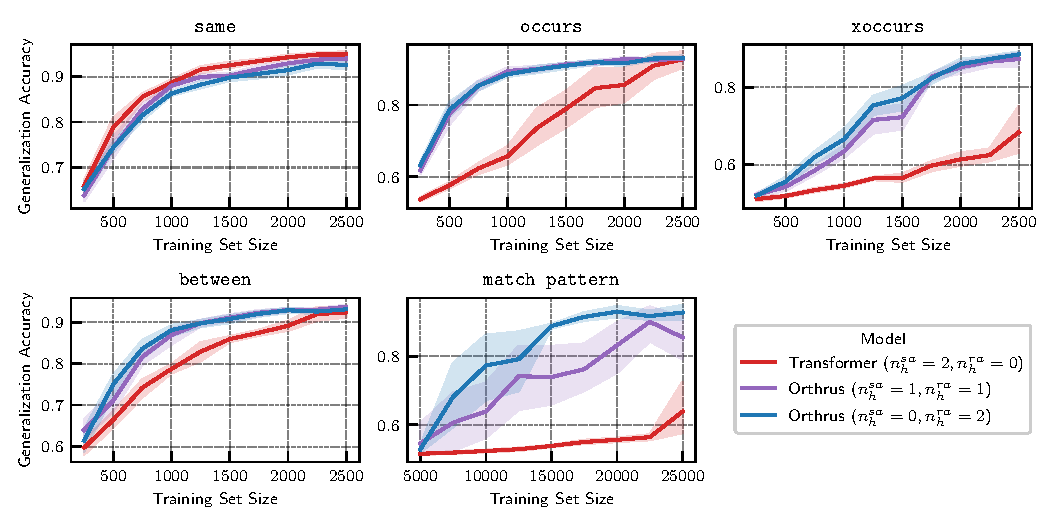
\includegraphics[width=\textwidth]{figs/experiments/relgames/relgames_learning_curves.pdf}
    \caption{Learning curves on the relational games benchmark. \textit{DAT} is more sample-efficient compared to a Transformer with the same total number of heads. Solid lines indicate the mean over 5 trials with different random seeds and the shaded regions indicate bootstrap 95\% confidence intervals.}\label{fig:relgames_learning_curves}
\end{figure}

In this experiment, we use positional symbols as the symbol assignment mechanism since the objects can be identified through their position on the grid. We also impose symmetry on the relations in relational attention, which we find to be a useful inductive bias. Intuitively, this is because the task-relevant relations are symmetric similarity relations across different visual attributes. We provide further discussion and present ablations in~\Cref{ssec:appendxi_relgames}.

\subsection{Improved Symbolic Reasoning in Sequence-to-Sequence tasks: Mathematical Problem Solving}\label{ssec:math}

Next, we evaluate \textit{DAT} on a set of mathematical problem-solving tasks based on the benchmark contributed by~\citet{saxtonAnalyzingMathematicalReasoning2019}. We use this as a proxy for ``symbolic reasoning''. Mathematical problem solving is an interesting test for neural models because it requires more than statistical pattern recognition---it requires inferring laws, axioms, and symbol manipulation rules. The benchmark consists of a suite of mathematical problem solving datasets, with each dataset consisting of a set of question-answer pairs. The tasks range across several modules or topics including solving equations, adding polynomials, expanding polynomials, differentiating functions, predicting the next term in a sequence, etc. For example, an example of question in the `\texttt{polynomials\_\_expand}' task is ``\texttt{Expand (5*x - 3) * (2*x + 1)}'' with the target ``\texttt{10 * x ** 2 - x - 3}''.

This is modeled as a sequence-to-sequence task with character-level encoding. We compare \textit{DAT} against a Transformer using matching encoder-decoder architectures. We use 2-Layer models with the total number of heads fixed to $8$ in both the encoder and the decoder. We compare an encoder-decoder Transformer with $\nhsa = 8$ against two configurations of \textit{DAT}: one with $\nhsa = \nhra = 4$ for the encoder and $\nhsa = 8, \nhra = 0$ for the decoder (config 1) and another with with $\nhsa = \nhra = 4$ for both the encoder and and decoder (config 2). The number of cross-attention heads is $8$ in all cases. The \textit{DAT} models use position-relative symbols as their symbol assignment mechanism.

\begin{figure}
    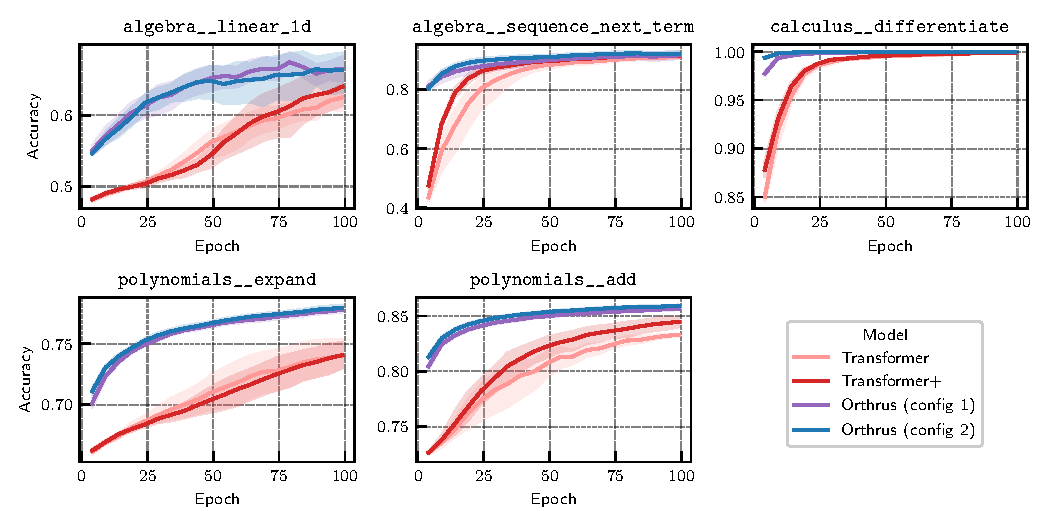
\includegraphics[width=\textwidth]{figs/experiments/math/math_training_curves_interpolation.pdf}
    \caption{Validation accuracy over the course of training on mathematical problem-solving tasks. \textit{DAT} learns faster and reaches higher accuracy. Solid lines indicate mean over 5 trials with different random seeds, and shaded regions indicate 95\% bootstrap confidence intervals.}\label{fig:math_training_curves_interpolation}
\end{figure}

Each model is trained for 100 epochs, and accuracy on a hold-out validation set is tracked over the course of training. For each model and task, we run 5 trials with different random seeds to compute approximate confidence intervals. We find that \textit{DAT} models learn faster and reach higher accuracies compared to a standard Transformer.

\subsection{Improvements in Language Modeling}\label{ssec:tiny_stories}

In this section, we evaluate \textit{DAT} on autoregressive language modeling. Transformer language models are typically built on what is sometimes called a ``decoder-only'' architecture. The model receives a sequence of tokens as input and is trained to causally predict the next token at each position.

We evaluate the language modeling capabilities of \textit{DAT}, as compared to standard Transformers, using the ``Tiny Stories'' dataset of~\citet{eldanTinyStoriesHowSmall2023}. The dataset consists of short stories and is intended as a benchmark for small language models. Again, for each configuration, we fix the total number of attention heads, and compare a Transformer with only standard self-attention heads to \textit{DAT} models with a mix of self-attention and relational attention heads. We compare a Transformer with $\nhsa = 8$ attention heads to two configurations of \textit{DAT}, one with $\nhsa = 6, \nhra = 2$ and another with $\nhsa = \nhra = 4$.

\begin{figure}[ht]
    \begin{subfigure}{0.33\textwidth}
        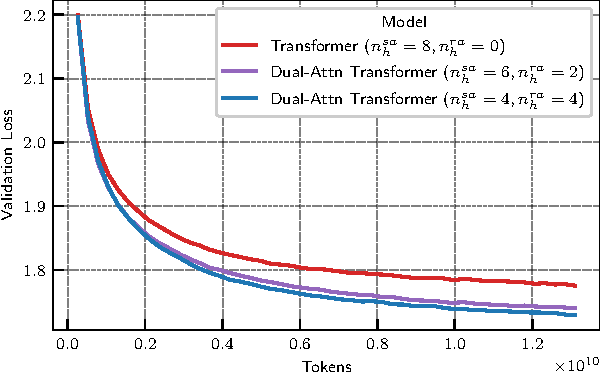
\includegraphics[width=\textwidth]{figs/experiments/tiny_stories/d64L4_symattn_asymra.pdf}
        \caption{4 Layers}
    \end{subfigure}
    \begin{subfigure}{0.33\textwidth}
        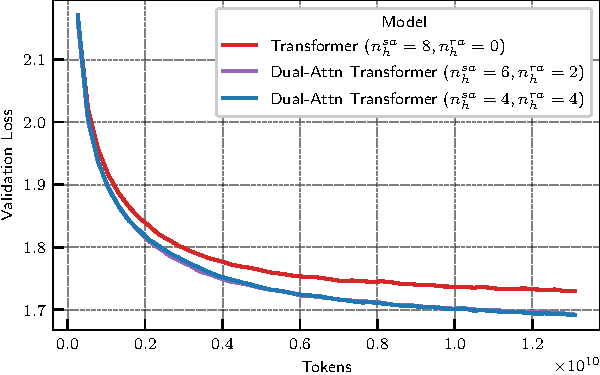
\includegraphics[width=\textwidth]{figs/experiments/tiny_stories/d64L5_symattn_asymra.pdf}
        \caption{5 Layers}
    \end{subfigure}
    \begin{subfigure}{0.33\textwidth}
        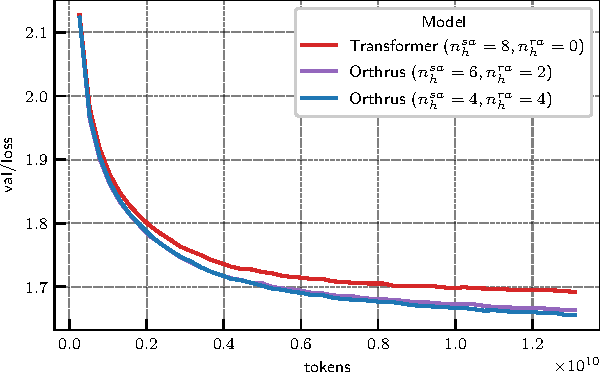
\includegraphics[width=\textwidth]{figs/experiments/tiny_stories/d64L6_symattn_asymra.pdf}
        \caption{6 Layers}
    \end{subfigure}
    \caption{Validation loss curves on a language modeling task. The $x$-axis indicates the number of tokens and the $y$-axis is the validation loss. \textit{DAT} achieves a smaller validation loss for the same total number of attention heads.}\label{fig:tiny_stories_val_loss_curves}
\end{figure}

\Cref{fig:tiny_stories_val_loss_curves} depicts the validation loss over the course of training for each model. We find that \textit{DAT} models with dual head attention achieve lower loss for the same total number of attention heads. We also varied the number of layers, and observed that the trend persists as the number of layers increases. The effect is small but consistent. The two \textit{DAT} configurations behave similarly, with perhaps a very slight advantage to $\nhsa = \nhra = 4$ (the configuration with a balanced composition of head types).

In~\Cref{fig:tiny_stories_val_loss_curves}, the \textit{DAT} models use \textit{symbolic attention} as the symbol assignmnet mechanism and asymmetric relations in relational attention. We find that symbolic attention outperforms position-relative symbols on this language modeling task. In fact, with position-relative symbols, there is no discernable advantage over the Transformer. Symbolic attention may be well-suited to language due to its implementation of a learned differentiable equivalence class mapping, which can perhaps be thought of as a form of syntax. We also find that asymmetric relations in relational attention perform better than symmetric relations. This may be because the relevant relations in language modeling are asymmetric (e.g., asymmetric syntactic or grammatical relations such as noun-verb, subject-object, determiner-noun, etc.). We provide further discussion and present ablations in~\Cref{ssec:appendix_lm}.

We conclude this section by noting that modern large language models are applied to diverse and multi-modal tasks, where different inductive biases will be useful in different contexts. While the language models explored in this section are small, an interesting avenue for future research would be to investigate whether the observed performance benefits scale up to larger models.

\subsection{The Benefits of Relational Inductive Biases in Vision: Image Recognition with ImageNet}\label{ssec:imagenet}

In the final set of experiments, we evaluate \textit{DAT} on a vision task---object classification with the ImageNet dataset~\citep{imagenet}. This further probes \textit{DAT}' ability in different modalities as a general-purpose sequence model. This section also stress tests \textit{DAT} at larger scales.

\begin{figure}[ht]
    \centering
    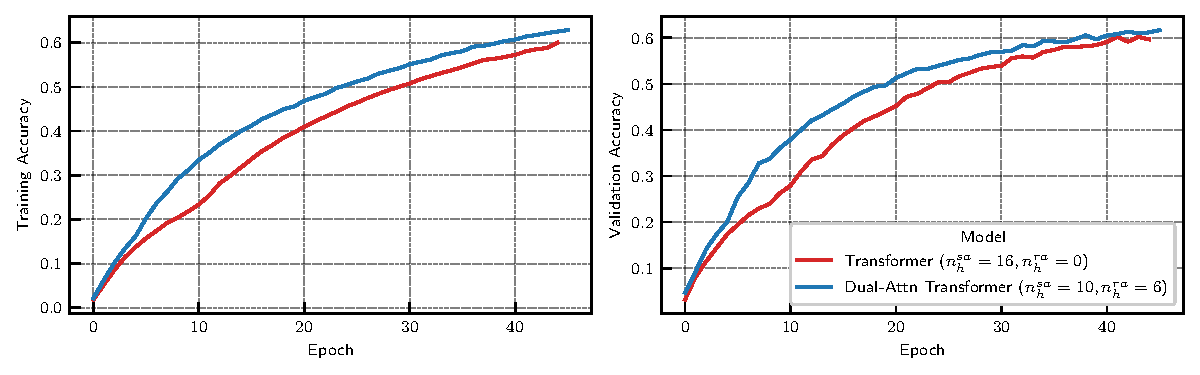
\includegraphics[width=0.9\textwidth]{figs/experiments/imagenet/imagenet_acc_curves.pdf}
    \caption{\textit{DAT} compared to a Vision Transformer on image recognition with ImageNet. \textit{DAT} learns faster and achieves better performance.}\label{fig:vision_acc_curve}
\end{figure}

Here, we again use a Vision Transformer-style architecture \citep{dosovitskiyImageWorth16x162020}. ImageNet's RGB images are divided into $16 \times 16$ patches, flattened, and linearly embedded into a vector. A learnable positional embedding is added to each patch embedding. We also prepend a special classification token. The sequence of patch embeddings are then fed through an Encoder and the embedding of the class token is used to generate the final classification through a fully connected layer. We compare a Vision Transformer model with $n_h^{sa} = 16$ to an \textit{DAT} model with $n_h^{sa} = 10, n_h^{sa} = 6$. For both, we used a model dimension $\dmodel = 1024$ and $L = 24$ layers. The \textit{DAT} model uses position-relative symbols as the symbol assignment mechanism and symmetric relational attention.

\Cref{fig:vision_acc_curve} depicts the training and validation accuracy over the course of training. We find that \textit{DAT} learns significantly faster. Averaging over epochs, \textit{DAT} has 5.0 (resp., 4.4) percentage points higher training accuracy (resp., validation accuracy) over the course of training compared to a standard Vision Transformer. At the end of training, \textit{DAT} maintains a 2.9 (resp., 1.5) percentage point advantage. This suggests that relational processing is important in processing visual scenes. This matches our intuition that parsing a visual scene requires reasoning about the visual relations between different objects or parts in the scene.

